
\begin{abstract}
    The computational sparsity of Mixture-of-Experts (MoE) models enables sub-linear growth in compute cost as
    model size increases, thus offering a scalable path to training massive neural networks.
    However, existing implementations suffer from low GPU utilization, significant latency overhead,
    and a fundamental inability to leverage task locality,
    primarily due to CPU-managed scheduling, host-initiated communication, and frequent kernel launches.
    To overcome these limitations, we develop~\sysname,
    a fully GPU-resident MoE operator that fuses expert computation and inter-GPU communication
    into a single persistent GPU kernel.
    \sysname enables fine-grained pipelining of dispatch, compute, and combine phases,
    eliminating launch overheads and reducing idle gaps.
    Unlike existing work, \sysname obviates bulk-synchronous collectives
    for one-sided, device-initiated, inter-GPU (R)DMA transfers, thus unlocking
    payload efficiency, where we eliminate bloated or redundant network
    payloads in sparsely activated layers.
    When evaluated on an 8-H100 GPU node with MoE models having up to 128 experts and 16K token sequences,
    \sysname achieves up to \textbf{9}$\times$ higher GPU utilization, \textbf{6}$\times$ lower latency,
    \textbf{5.7}$\times$ higher throughput, and \textbf{4}$\times$ better overlap efficiency
    compared to state-of-the-art baselines—despite using FP32 while baselines use FP16.
    \sysname shows that principled GPU kernel-hardware co-design
    is key to unlocking the performance ceiling of large-scale distributed ML\@.
\begin{figure}[!h]
    \centering
    \begin{subfigure}{0.4\textwidth}
        \centering
        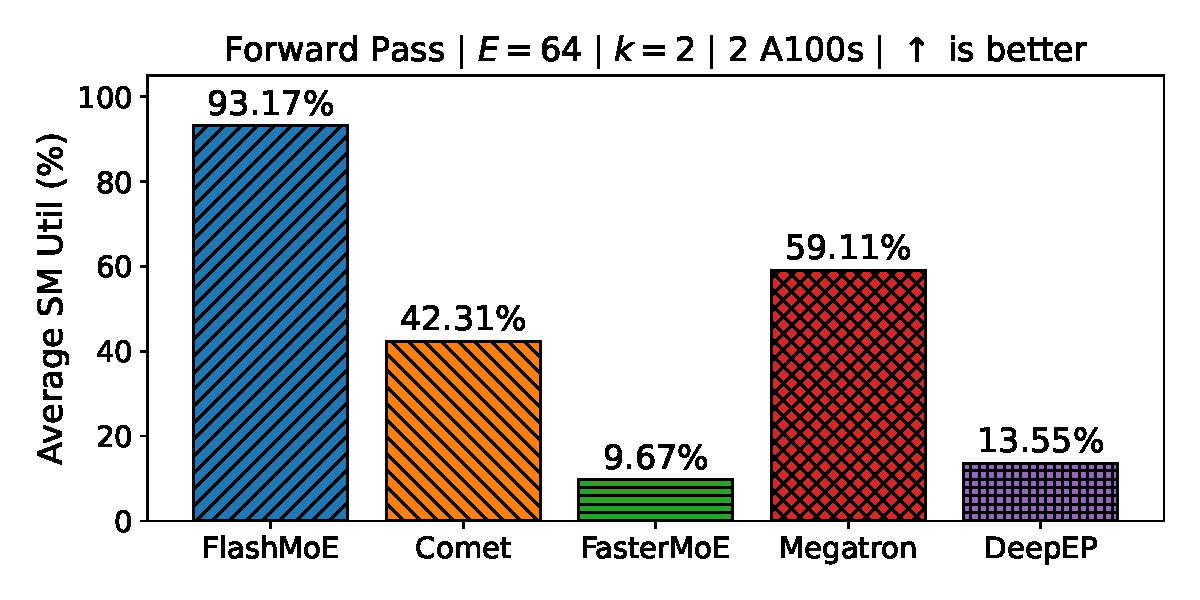
\includegraphics[width=\linewidth, keepaspectratio]{flash_figs/sm_util}
        \caption{GPU SM Utilization}
        \label{sub:e}
    \end{subfigure}
    \begin{subfigure}{0.4\textwidth}
        \centering
        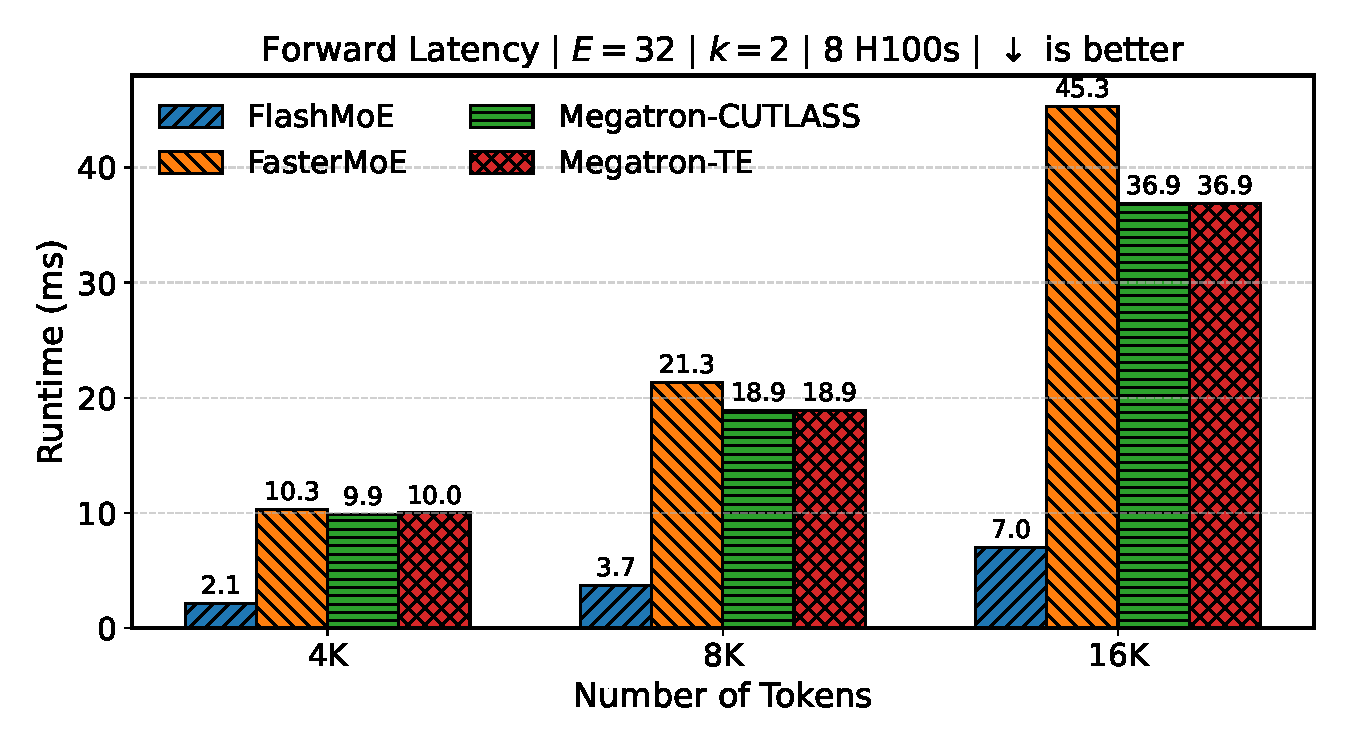
\includegraphics[width=\linewidth, keepaspectratio]{flash_figs/scaling_tokens_8}
        \caption{Scaling Tokens}
        \label{sub:r}
    \end{subfigure}
    \begin{subfigure}{0.4\textwidth}
        \centering
        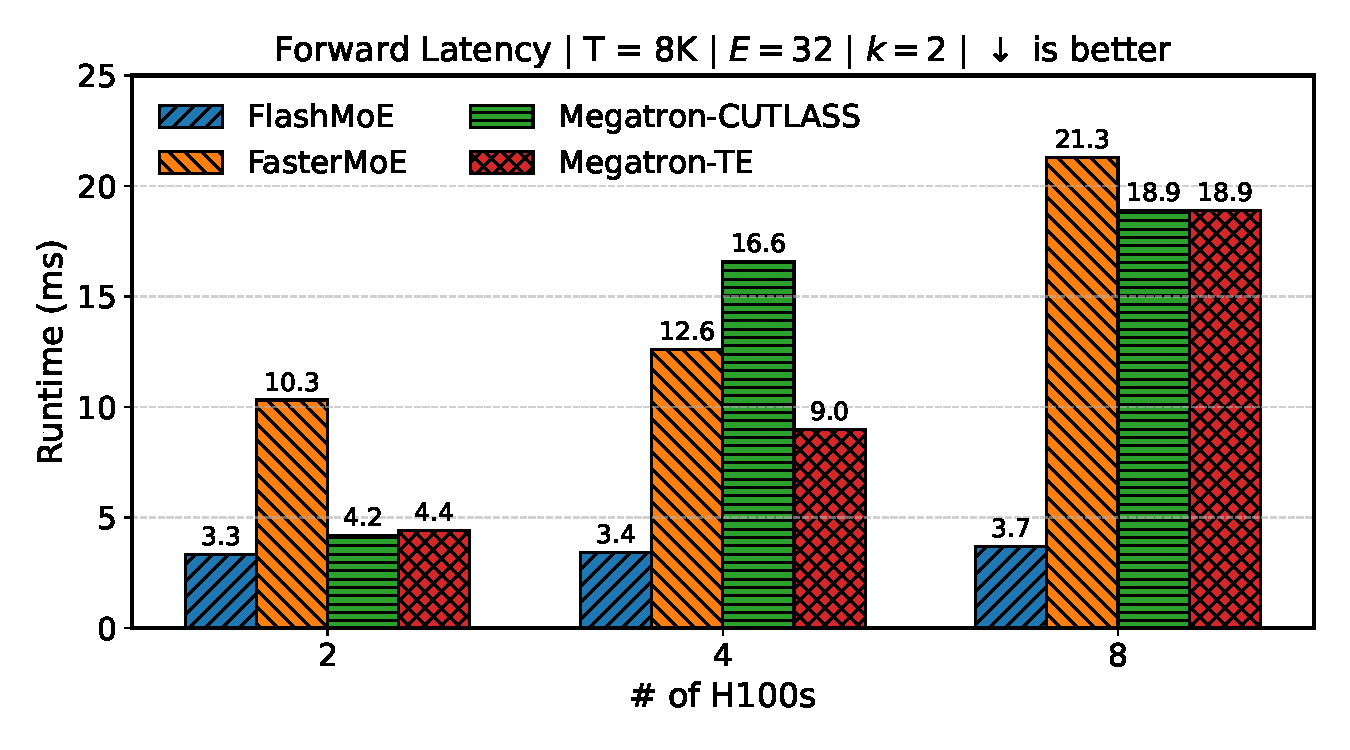
\includegraphics[width=\linewidth, keepaspectratio]{flash_figs/scaling_gpus_8}
        \caption{Weak Scaling across GPUs}
        \label{sub:e1}
    \end{subfigure}
    \begin{subfigure}{0.4\textwidth}
        \centering
        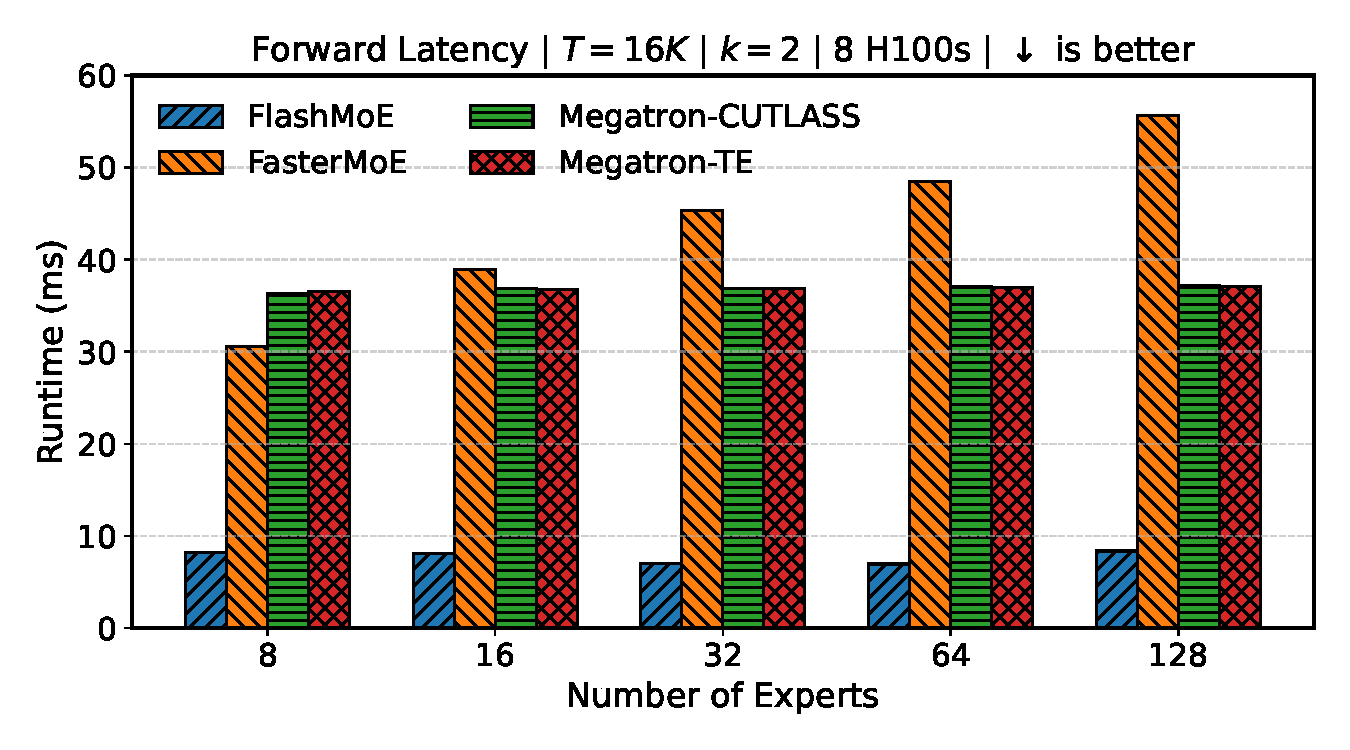
\includegraphics[width=\linewidth, keepaspectratio]{flash_figs/scaling_experts_8}
        \caption{Across Experts}
        \label{sub:r2}
    \end{subfigure}
    \caption{\sysname performance.}
    \label{fig:str}
\end{figure}
\end{abstract}